%\documentclass[12pt,letterpaper,twoside]{article}
\documentclass[12pt,letterpaper]{article}
\usepackage{amsmath}
\usepackage{amsfonts}
\usepackage{appendix}
\usepackage[figurewithin=section,tablewithin=section]{caption}
\usepackage[usenames,dvipsnames]{color}
\usepackage{graphicx}
\usepackage{longtable}
\usepackage{rotating}
%\usepackage{verbatim}
\usepackage[pdftex,bookmarksopen=false]{hyperref}
%\usepackage[pdftex]{hyperref}
\hypersetup{pdfauthor={John Sibert}}
\hypersetup{pdfsubject={Yellowfin stock assessment}}
\hypersetup{pdftitle={Assessment of the yellowfin tuna Thunnus albacares 
stock in the Main Hawaiian Islands Yellowfin Tuna Fishery}}
\hypersetup{pdfkeywords={yellowfin tuna,state space model,stock assessment,Hawaii}}

\newcommand\doublespacing{\baselineskip=1.6\normalbaselineskip}
\newcommand\singlespacing{\baselineskip=1.0\normalbaselineskip}
\renewcommand\deg[1]{$^\circ$#1}
\newcommand\SD{SEAPODYM}
\newcommand\MFCL{MULTIFAN-CL}
\newcommand\ADMB{ADModel Builder}
\newcommand\SPC{Secretariat of the Pacific Community}
\newcommand\WCPO{Western Central Pacific Ocean}
\newcommand\WCPFC{Western Central Pacific Fisheries Commission}
\newcommand\SSAP{Skipjack Survey and Assessment Programme}
\newcommand\RTTP{Regional Tuna Tagging Programme}
\newcommand\PTTP{Pacific Tuna Tagging Programme}
\newcommand\FAD{fish aggregating device}
\newcommand\ADRM{advection-diffusion-reaction model}
\newcommand\help[1]{\color{Magenta}{\it #1}\normalcolor}
\newcommand\widebar[1]{\overline{#1}}
\newcommand\EEZ{Exclusive Economic Zone}

\newcommand\None{{N_{1,1}}}
\newcommand\Ntwo{{N_{2,1}}}
\newcommand\Nsum{{N_{1,1}+N_{2,1}}}
\newcommand\peryr{yr$^{-1}$}
\newcommand\prevN[1]{{#1_{t-\Delta t}}}
\newcommand\nextN[1]{{#1_t}}
\newcommand\MSY{\widetilde{Y}}
\newcommand\Fmsy{F_{\MSY}}
\newcommand\MSYFmsy{\MSY\;\Fmsy}
\newcommand\Bd{B_1\; d}

\title{Assessment of the yellowfin tuna ({\it Thunnus albacares}) 
stock in the Main Hawaiian Islands Yellowfin Tuna Fishery}

\author{
John Sibert\thanks{sibert@hawaii.edu}\\
Joint Institute of Marine and Atmospheric Research\\
University of Hawai'i at Manoa\\
Honolulu, HI  96822 U.S.A.\\[0.125in]
\date{\today}
}

%\pagestyle{myheadings}
%\markboth{John Sibert\hfil MHI Yellowfin Assessment}
%{MHI Yellowfin Assessment Model\hfil John Sibert}

\pagestyle{headings}
\markright{MHI Yellowfin Assessment Model\hfil John Sibert}

\begin{document}
% amsmath package
%\numberwithin{equation}{section}
%\numberwithin{figure}{section}
\maketitle

\doublespacing

\begin{abstract}
\begin{center}\help{Write me!}\end{center}
\end{abstract}


\section*{Introduction}
The responsibility to manage fisheries for tunas and tuna-like species
lies regional organizations established under international treaties.
In the Western Central Pacific Ocean, this responsibility devolves to
the Western and Central Pacific Fisheries Commission (WCPFC, 
\url{https://www.wcpfc.int}).
The WCPFC conducts stock assessments for several species of tunas and
implements fishery management and conservation measures based on
these stock assessments. The WCPFC stock assessments provide estimates
of stock size and indicators of productivity of the WCPFC area of
responsibility, but offer little advice to local fishery managers about
the extent that local small-scale fisheries are effecting local
populations.

Yellowfin tuna ({\it Thunnus albacares}) is an important food resource
of many Pacific Island communities and the people of the Hawaiian
islands of been fishing for yellowfin for many generations. 
The Main Hawaiian Islands (MHI), Figure~\ref{fig:mhimap},
comprising the 8 largest islands in the Hawaiian Archipelago
has been an important fishing ground throughout this history.
(Indeed, since the creation of the Papah\={a}naumoku\={a}kea Marine National
Monument in 2016, it is the only legally accessible tuna fishing ground
in the State of Hawaii.)
The State of Hawaii has collected yellowfin catch data from the MHI
since 1949, but these data have never been analyzed in a formal stock
assessment.

This paper presents an assessment of the stock of yellowfin tuna
residing in the MHI that may be of use to fishery managers in Hawaii
in addressing questions about the effects of the fishery on the
population. The general approach is to adopt a state-space surplus
production model  (Schaefer, 1954). The model has several
novel features.
Fishing mortality, the proportion of the population harvested each
year, is represented as a random walk (Nielsen and Berg, 2014).
Biomass estimates from the 2014 WCPFC yellowfin stock assessment
(Davies, et al. 2014) can be used as indices of abundance.
The logistic component of the surplus production model is
reparameterized to estimate parameters of direct relevance to fishery
management.

\begin{figure}
\begin{center}
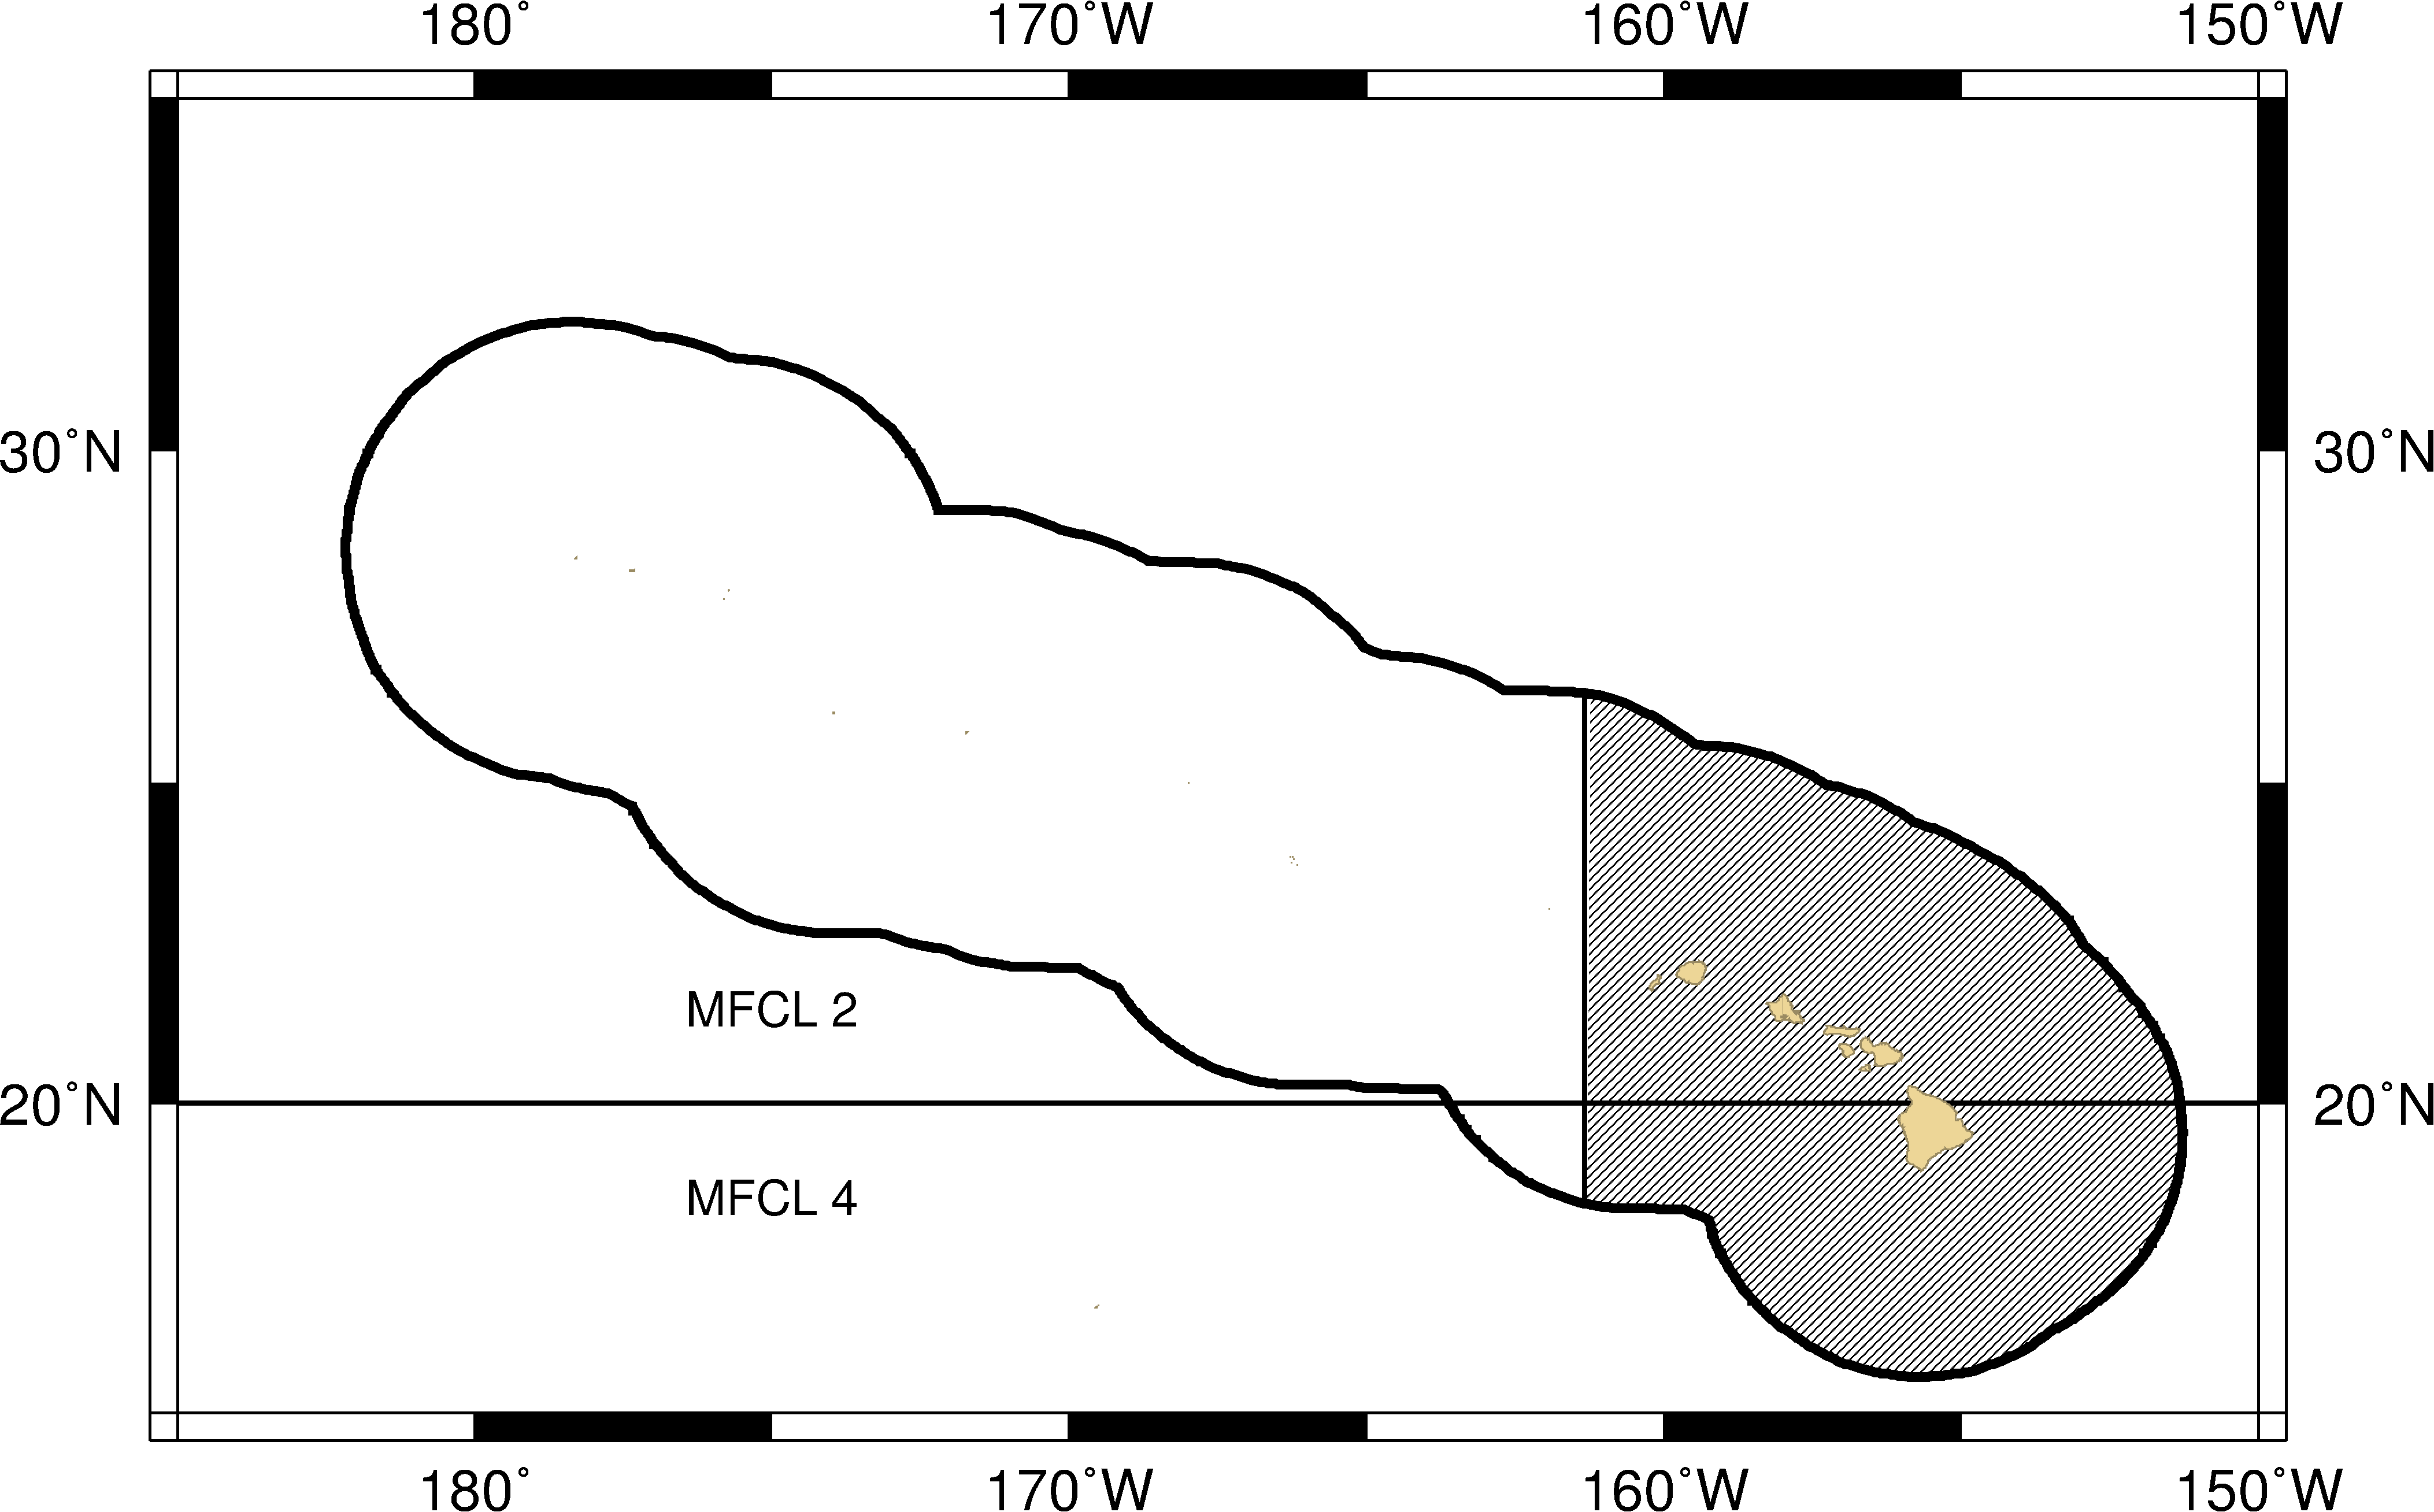
\includegraphics[width=\textwidth]{./graphics/HI_regions.png}
\caption{\label{fig:mhimap}
The United States Exclusive Economic Zone around the Hawaiian
Archipelago. The Main Hawaiian Islands lie in the shaded area at the
extreme east of the EEZ. The line at 20\deg{N} latitude is the
boundary between WCPFC stock assessment regions 2 and 4. See text for
full explanation.
}
\end{center}
\end{figure}

\section*{References}
{\parindent=0cm \small
\everypar={\hangindent=2em \hangafter=1}\par
%\doublespacing
Carruthers, T. and M. McAllister. 2011.
Computing prior probability distributions for the
intrinsic rate of increase for Atlantic tuna and
billfish using demographic methods.
Collect. Vol. Sci. Pap. ICCAT, 66(5): 2202-2205.

Davies, N., S. Harley, J. Hampton, S. McKechnie. 2014. Stock
assessment of yellowfin tuna in the western and central pacific ocean.
WCPFC-SC10-2014/SA-WP-04.

Fournier, D. A., H.J. Skaug, J. Ancheta, J.Sibert, J. Ianelli, 
A. Magnusson, M. N. Maunder, A. Nielsen. 2012. AD Model Builder:
using automatic differentiation for for statistical inference of highly
parameterized complex nonlinear models. Optimization Methods and
Software 27, 233–249.

Nielsen, A., C. Berg. 2014. Estimation of time-varying selectivity
in stock assessments using state-space models. Fisheries Research
158:96-101.

Murray, J. D. 1993. Mathematical biology. Second Edition.
Springer-Verlag. 767pp.

Quinn, T, R. Deriso. 1999. Quantitative fish dynamics. Oxford
University Press, New York.

Schaefer, M. B. 1954. Some aspects of the dynamics of populations
important to the management of the commercial marine fisheries. IATTC
Bull. 1(2):27-56.

Senina, I., J. Sibert, P. Lehodey  2008. Parameter estimation for
basin-scale ecosystem linked population models of large pelagic
predators: Application to skipjack tuna.  Prog. Oceanogr. 78:319-335.

Sibert, J. R. 2015. Feasibility of developing a stock assessment
model for Main Hawaiian Islands Yellowfin Tuna Fishery.
119th Meeting of the Scientific and Statistical Committee.
Document 7.A.1(1)Rev 1.

Skaug, H., Fournier, D., 2006. Automatic approximation of the marginal
likelihood in non-Gaussian hierarchical models. Computational
Statistics \& Data Analysis 51, 699–709.

Wells, D., J. Rooker, D. Itano. 2012.  Nursery origin of yellowfin
tuna in the Hawaiian Islands. Mar. Ecol. Prog. Ser. 461:187-196. 
\par}


 
\end{document}

Regulation of catches of tunas by fisheries in the waters surrounding
the Hawaiian Islands is the responsibility of the Western and Central
Pacific Fisheries Commission (WCPFC).
The WCPFC conducts stock assessments for the region over which it has
jurisdiction. These assessments provides estimates of stock size and
productivity which with Commission uses to set fishery management
policy, but offers little guidance applicable to small scale
fisheries.
%This international legal arrangement is intended to regulate large
%scale fisheries for tunas, 
